\documentclass[10pt,twocolumn]{article}

\usepackage[letterpaper,margin=0.82in,columnsep=0.28in]{geometry}
\usepackage{graphicx}
\usepackage{booktabs}
\usepackage{amsmath,amssymb}
\usepackage[dvipsnames]{xcolor}
\usepackage{caption}
\usepackage{titlesec}
\usepackage{authblk}
\usepackage{tikz}
\usetikzlibrary{arrows.meta,positioning,fit,backgrounds,calc}
\usepackage[hidelinks]{hyperref}

\definecolor{ink}{HTML}{17211C}
\definecolor{accent}{HTML}{AF4A2C}
\definecolor{field}{HTML}{2C6E52}
\definecolor{steel}{HTML}{3B6E8F}
\definecolor{paper}{HTML}{EEF1EC}
\color{ink}
\captionsetup{font=small,labelfont=bf,labelsep=period}
\titleformat{\section}{\normalfont\large\bfseries\color{ink}}{\thesection}{0.6em}{}
\titleformat{\subsection}{\normalfont\normalsize\bfseries\color{ink}}{\thesubsection}{0.5em}{}
\titlespacing*{\section}{0pt}{1.2ex}{0.6ex}
\titlespacing*{\subsection}{0pt}{0.9ex}{0.4ex}
\setlength{\parskip}{0.15ex}
\renewcommand{\arraystretch}{1.12}

% tikz styles for the schematics
\tikzset{
  blk/.style={draw=ink,rounded corners=2pt,fill=paper,align=center,inner sep=3.2pt,font=\scriptsize,minimum height=6.2mm},
  sel/.style={draw=field,line width=0.9pt,rounded corners=2pt,fill=field!12,align=center,inner sep=3.2pt,font=\scriptsize,minimum height=6.2mm},
  obox/.style={draw=accent,rounded corners=2pt,fill=accent!10,align=center,inner sep=3.2pt,font=\scriptsize,minimum height=6.2mm},
  fl/.style={-{Stealth[length=4pt]},draw=ink!70,line width=0.6pt},
}

\title{\vspace{-3.5ex}\textbf{\large DiamondWorld: A Market-Validated Causal Simulator\\[-0.2ex] for Baseball Games}}
\author[1]{Luke Blommesteyn}
\author[2]{Jaden Majumdar}
\affil[1]{\normalsize\textnormal{Western University\quad\texttt{lblommes@uwo.ca}}}
\affil[2]{\normalsize\textnormal{University of Toronto\quad\texttt{jaden.majumdar@mail.utoronto.ca}}}
\date{\vspace{-3ex}\small MIT Sloan Sports Analytics Conference, Research Paper Track}

\begin{document}
\twocolumn[
\begin{@twocolumnfalse}
\maketitle
\begin{abstract}
\noindent
Projection systems answer \emph{how good is a player}. They cannot answer \emph{what happens in this
game}, because a game is a correlated sequence of plate appearances, not a sum of independent rates.
We present DiamondWorld, a plate-appearance-level generative model, an empirical rules engine, and a
full game simulator that plays out complete games one plate appearance at a time. This makes it a tool
for questions projection systems are structurally unable to touch: counterfactual what-ifs, lineup
construction, correlated tail-risk, and win probability with honest uncertainty. Our central
contribution is not the simulator but its \emph{validation}. We show that the simulator's causal
what-if estimates match how an independent, information-aggregating market prices the same games. Using
a leak-free natural experiment (within a series the two teams are fixed, so the game-to-game change in
the market-implied win probability is driven by the starter and lineup, exactly what a counterfactual
isolates), the simulator's within-series win-probability deltas correlate $r{=}0.32$ with the market's
on both pitching and hitting changes, using no game outcomes. The agreement holds a full season
out-of-sample ($r{=}0.33$ on a season the model's rates predate) and against a second, independent
market source. Calibrating the simulator's causal magnitudes to the market yields effects that agree in
both direction and size. We ground the object with benchmarks that are honest about where it does and
does not lead: its per-game run distribution is well calibrated (interval coverage $0.54/0.82/0.90$
against nominal $0.50/0.80/0.90$) where a summed model badly under-covers, while its point win
probability is calibrated but less sharp than a simple team-strength baseline. To our knowledge this is
the first market-validated causal simulator for baseball.
\vspace{1.4ex}
\end{abstract}
\end{@twocolumnfalse}
]

\section{Introduction}
Player projection is a solved-enough problem. Steamer, ZiPS, THE\,BAT, and Marcel~\cite{tango} each map
a player to expected rates, and they agree closely. A front office, though, rarely asks only \emph{how
good is this player}. It asks \emph{what does acquiring this pitcher do to our playoff chances},
\emph{does this lineup change the shape of tonight's game}, \emph{how confident should we be in this
win probability}. These are causal and distributional questions about a specific game, and a projection
system, even summed over nine hitters, cannot answer them, because a game is a correlated sequence of
plate appearances (PAs). A walk, a single, and a home run cluster in one inning. The mean is a sum of
rates; the \emph{shape} is not.

A generative game simulator can answer these questions by construction. The difficulty has never been
building one. It is trusting it. A simulator will happily report that swapping in an ace is worth $9.8$
points of win probability, but that number is internally generated, and it could be an artifact of a
generic bullpen, a crude lineup model, or a miscalibrated player prior. The contribution of this paper
is to close that gap. We validate the simulator's \emph{causal} estimates against an external ground
truth, namely how an information-aggregating market prices real games when a single input changes, and
we do so leak-free, out-of-sample across seasons, and against more than one independent market source.
The simulator that survives this test is a decision tool, not a demo.

\section{Related work}
\textbf{Player projection.} Systems such as Marcel~\cite{tango}, Steamer, ZiPS, and THE\,BAT regress
weighted recent performance toward a population mean. They are accurate and mutually consistent, and we
benchmark against Marcel (the reproducible baseline the others are measured against) and Steamer's real
releases. By design they are marginal, and do not model a specific game.

\textbf{Game simulation and Markov models.} Markov-chain models of baseball~\cite{bukiet} compute run
distributions and optimal orders from state-transition probabilities, and are the lineage of our
empirical rules engine. Recent work simulates counterfactual hitting strategies with deep
models~\cite{nakahara}. Our contribution relative to these is not the simulator but the external,
market-based validation of its causal outputs.

\textbf{Game-state value models.} The closest methodological relatives are continuous game-state value
models, most prominently expected possession value in basketball~\cite{cervone}, which estimate the
value of a game state from a stochastic process. Like that work we produce game-state-conditional
estimates; unlike it, our targets are discrete counterfactual interventions, and we validate them
against an independent market.

\textbf{Self-supervised representation learning.} Our evaluation note (\S\ref{sec:arch}) concerns
joint-embedding predictive architectures~\cite{lecun,assran} trained with variance-covariance
regularization~\cite{bardes}. We find that on a saturated-likelihood problem a frozen probe minimizes
held-out loss while discarding the very structure a world model needs.

\textbf{Evaluation.} We use proper scoring rules and probability-integral-transform
calibration~\cite{gneiting} for the distributional benchmarks, and classical win-probability baselines,
Log5 and the Pythagorean expectation~\cite{james}, as the team-strength reference. To our knowledge, no
prior work validates a causal baseball game simulator against how an independent market prices real
games.

\section{The DiamondWorld model}
DiamondWorld is a pipeline of three components (Fig.~\ref{fig:system}). The \textbf{plate-appearance
model} is a stochastic-variational generative model~\cite{phan,jax} that emits each PA's outcome as a
nine-way categorical (K, BB, HBP, 1B, 2B, 3B, HR, out, reached-on-error) conditioned on batter and
pitcher identity, park, and game state. Player identity enters through a learned skill latent plus
recency-weighted rate features. Two modeling choices matter for the results below. First, correcting a
minibatch scaling of the skill-latent divergence revived a posterior that had collapsed to its prior,
lifting cross-player differentiation substantially. Second, the current model adds \emph{contact-quality
features}: expected hit and home-run rates built by binning every batted ball on exit velocity and
launch angle and reading the league outcome frequency in each bin (Fig.~\ref{fig:heat}). This was the
single largest input lever we found (\S\ref{sec:bench}).

\begin{figure}[t]
\centering
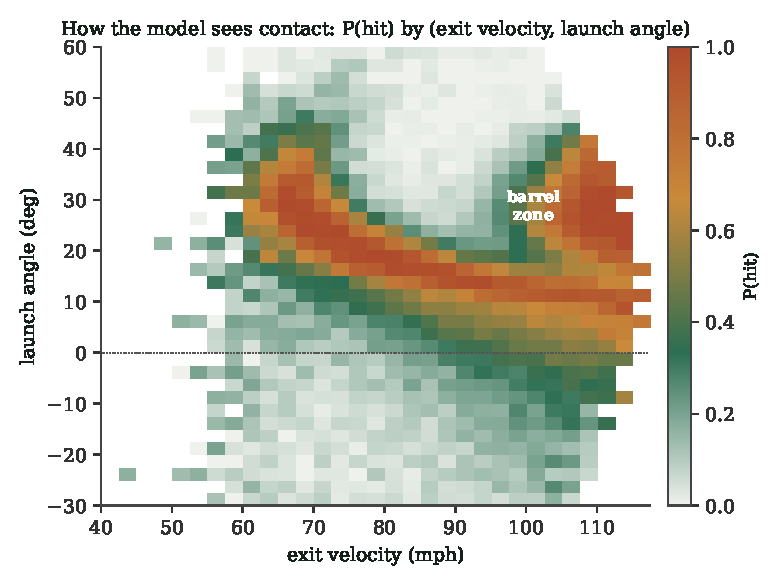
\includegraphics[width=\linewidth]{figs/fig6_heatmap.pdf}
\caption{The contact-quality feature. League probability of a hit as a function of exit velocity and
launch angle, built directly from batted-ball data. The bright band is the barrel zone. Scoring a
batter on the quality of contact made, rather than on which balls happened to fall in, is what lets the
model separate skill from ball-in-play luck.}
\label{fig:heat}
\end{figure}

The \textbf{empirical rules engine} turns an outcome sequence into runs and base-state transitions.
Ported from a validated Markov baseline~\cite{bukiet}, it reproduces test-season run totals to within
half a percent, so the run-scoring problem reduces to getting per-PA outcomes right. The \textbf{game
simulator} plays full nine-inning-plus-extras games with lineup cycling, a bullpen, walk-offs, and the
ghost-runner rule. Relievers are governed by a fitted \emph{hook model}, a logistic hazard for pulling
the starter as a function of batters faced, times through the order, and runs allowed (held-out AUC
$0.889$), so bullpen usage is endogenous and uses only pre-game information. The model is trained on
2015--2023 (rates through 2024 for the out-of-sample season test) and evaluated on 2024 unless stated.

\begin{figure*}[t]
\centering
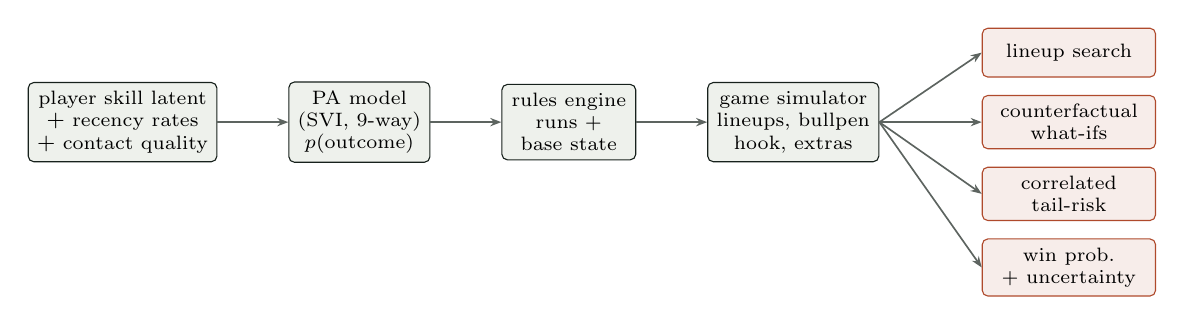
\begin{tikzpicture}[node distance=8mm and 9mm]
\node[blk,minimum width=20mm] (feat) {player skill latent\\ {\footnotesize +} recency rates\\ {\footnotesize +} contact quality};
\node[blk,right=of feat,minimum width=17mm] (pa) {PA model\\ {\scriptsize (SVI, 9-way)}\\ $p(\text{outcome})$};
\node[blk,right=of pa,minimum width=17mm] (eng) {rules engine\\ {\scriptsize runs +}\\ {\scriptsize base state}};
\node[blk,right=of eng,minimum width=19mm] (sim) {game simulator\\ {\scriptsize lineups, bullpen}\\ {\scriptsize hook, extras}};
\node[obox,right=13mm of sim,minimum width=22mm] (o1) {counterfactual\\ what-ifs};
\node[obox,above=2.2mm of o1,minimum width=22mm] (o0) {lineup search};
\node[obox,below=2.2mm of o1,minimum width=22mm] (o2) {correlated\\ tail-risk};
\node[obox,below=2.2mm of o2,minimum width=22mm] (o3) {win prob.\\ {\scriptsize + uncertainty}};
\draw[fl] (feat)--(pa); \draw[fl] (pa)--(eng); \draw[fl] (eng)--(sim);
\draw[fl] (sim.east)--(o0.west); \draw[fl] (sim.east)--(o1.west);
\draw[fl] (sim.east)--(o2.west); \draw[fl] (sim.east)--(o3.west);
\end{tikzpicture}
\caption{The DiamondWorld pipeline. A generative plate-appearance model provides outcome probabilities;
a validated rules engine converts outcomes to runs and base states; a full game simulator adds lineups,
an endogenous bullpen, and extras. Because the object is generative, four families of decision outputs
fall out directly.}
\label{fig:system}
\end{figure*}

\section{Architectures we evaluated}
\label{sec:arch}
We tested the generative model against the standard discriminative and self-supervised alternatives on
the same inputs and the same task (Fig.~\ref{fig:arch}): a per-PA MLP, a recurrent GRU over the PA
sequence, a causal transformer, and a joint-embedding predictive architecture (JEPA)~\cite{lecun,assran}
with variance-covariance regularization~\cite{bardes} and a frozen linear probe.

The natural metric, held-out per-PA log-likelihood, is the \emph{wrong} yardstick, and following it
selects the wrong model. A single PA is near maximum entropy (about $1.495$ nats), so every model scores
near the floor, and log-likelihood rewards getting the league-average distribution right, not telling
players apart, which is the whole job of a world model. The sharpest illustration is JEPA: with a frozen
probe it attains the best held-out likelihood and best raw accuracy of any model and near-zero player
differentiation (Fig.~\ref{fig:metric}). Two further findings sharpen the lesson. Fine-tuning JEPA's own
encoder end-to-end lifts player differentiation from $0.06$ to $0.54$, and training the identical encoder
from scratch does marginally better ($0.56$), so the collapse is the frozen self-supervised objective and
the pretraining itself adds nothing here. And once differentiation is measured correctly, architecture
barely matters: the transformer, GRU, and MLP all land near $0.577$. The lever that moves the number is
\emph{features}, not a fancier network, which is why the generative model with contact-quality features
leads. The takeaway for anyone building a generative sports model: pick the evaluation that matches the
use, or the best-scoring model will be the wrong one.

\begin{figure*}[t]
\centering
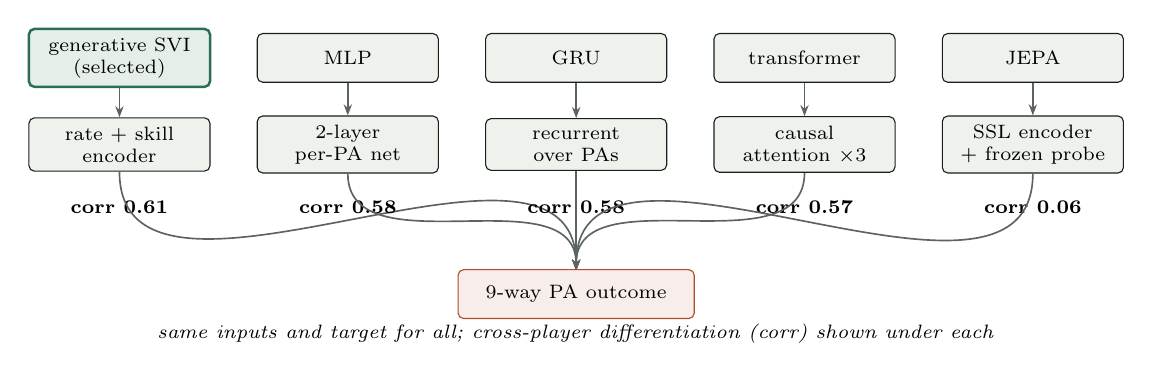
\begin{tikzpicture}[x=29mm,y=1mm]
\foreach \i/\name/\top/\mid/\corr/\st in {
  0/svi/{generative SVI\\ \scriptsize(selected)}/{rate + skill\\ encoder}/{corr 0.61}/sel,
  1/mlp/{MLP}/{2-layer\\ per-PA net}/{corr 0.58}/blk,
  2/gru/{GRU}/{recurrent\\ over PAs}/{corr 0.58}/blk,
  3/tfm/{transformer}/{causal\\ attention $\times3$}/{corr 0.57}/blk,
  4/jep/{JEPA}/{SSL encoder\\ + frozen probe}/{corr 0.06}/blk} {
  \node[\st,minimum width=23mm] (\name t) at (\i,0) {\top};
  \node[blk,minimum width=23mm] (\name m) at (\i,-11) {\mid};
  \node[font=\scriptsize\bfseries] at (\i,-19) {\corr};
  \draw[fl] (\name t)--(\name m);
  \draw[fl] (\name m) to[out=-90,in=90] (2,-27);
}
\node[obox,minimum width=30mm] at (2,-30) {9-way PA outcome};
\node[font=\scriptsize,align=center] at (2,-35)
  {\emph{same inputs and target for all; cross-player differentiation (corr) shown under each}};
\end{tikzpicture}
\caption{Architectures evaluated on identical inputs and the identical per-PA target. The generative
SVI with contact-quality features leads on player differentiation; discriminative nets cluster near
$0.58$; a frozen self-supervised JEPA probe collapses to $0.06$ despite the best likelihood
(Fig.~\ref{fig:metric}). Architecture is not the lever; features are.}
\label{fig:arch}
\end{figure*}

\section{What the simulator answers}
Because the object is generative, four families of questions fall out directly (Table~\ref{tab:cap}).
On one competitive 2024 game with $R{=}400$ replicas per scenario: counterfactuals (swapping the home
starter for a replacement arm, or upgrading the weakest hitter to a star bat, move win probability and
the full run distribution, as causal re-simulations of the same game); lineup construction (reordering
the same nine hitters moves expected runs by about $0.48$ across 40 orders, and the best beats the order
used by $0.27$ runs per game); correlated tail-risk (the simulated game-total variance is $1.98\times$
that of an independent-Poisson model with the same mean, exactly the within-game correlation a summed
model misses); and win probability with uncertainty (a generative model separates game randomness from
roster uncertainty, which over the full 2024 season are comparable in size, $4.6\%$ versus $4.9\%$ WP,
so a point estimate hides half the story). These capabilities are the product. Their credibility rests
on the next section.

\begin{table}[t]
\centering\footnotesize
\setlength{\tabcolsep}{4.5pt}
\caption{What each approach can answer. Only a full generative simulator delivers game-specific
correlated distributions, uncertainty decomposition, and \emph{validated} single-input counterfactuals.}
\label{tab:cap}
\begin{tabular}{@{}lccc@{}}
\toprule
\textbf{Capability} & \textbf{Proj.} & \textbf{Markov} & \textbf{DiamondWorld}\\
& \textbf{sum} & \textbf{run model} & \\
\midrule
Player rate lines & \checkmark & & \checkmark\\
Game-specific mean & partial & \checkmark & \checkmark\\
Correlated run distribution & & partial & \checkmark\\
Uncertainty decomposition & & & \checkmark\\
Lineup-order effect & & \checkmark & \checkmark\\
Single-input counterfactual & & & \checkmark\\
\;\;\emph{market-validated} & & & \checkmark\\
\bottomrule
\end{tabular}
\end{table}

\section{Validating the causal engine}
\label{sec:val}
The counterfactual estimate ``swap this starter, win probability moves by $X$'' has always been
internally generated. We check it against an external ground truth: an information-aggregating market's
implied win probability for the same teams under different pitchers. The natural experiment is a series.
Within a series the two teams and home field are fixed, so the game-to-game change in the market-implied
win probability is driven by the starter, lineup, and rest, exactly what a counterfactual isolates. If
the simulator's within-series win-probability deltas track the market's, the causal estimates have
external support that uses \emph{no game outcomes and no look-ahead} (Fig.~\ref{fig:series}).

\begin{figure}[t]
\centering
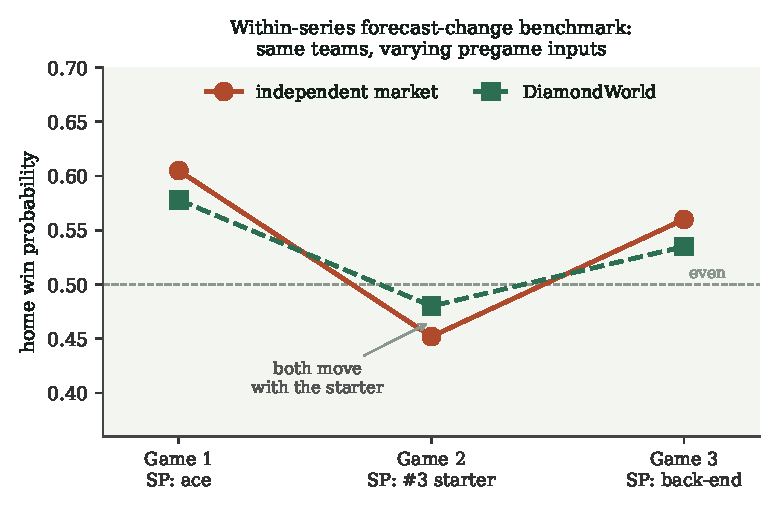
\includegraphics[width=\linewidth]{figs/fig8_series.pdf}
\caption{The within-series natural experiment (illustrative). Across a series the two teams and home
field are held constant, so the game-to-game move in win probability is the starter and lineup effect,
precisely a counterfactual. The validation measures whether the simulator's move (green) tracks the
independent market's (orange). It does, at $r{=}0.32$ leak-free.}
\label{fig:series}
\end{figure}

\textbf{Direction is validated, leak-free.} We residualize the simulator's and the market's logit win
probability against team fixed effects (team identity only, no outcomes) and correlate the residuals:
$r{=}0.33$. The within-series design (Fig.~\ref{fig:val}) gives $r{=}0.32$, significant far beyond a
permutation null (95th percentile $0.032$). The simulator's game-specific signal agrees with the market
beyond team strength, so it is capturing real starter and matchup effects the market also prices, not
noise.

\textbf{Magnitude is overstated, and we calibrate it.} The within-series slope of market on simulator is
$0.27$; correcting for the simulator's residual replica-sampling noise (reliability $0.80$ at $R{=}500$)
gives $0.33$. The raw simulator over-reacts to a single starter change by roughly $3\times$: a raw
$9.8$-point ace swap is about $3.3$ points in market-calibrated units. The result is a
\emph{market-calibrated} causal engine, with direction and magnitude both tied to an external ground
truth, and it corrects the raw headline numbers downward, which is the point of validating rather than
asserting.

\textbf{It is broad, not pitcher-only.} Within a series both the starter and the lineup change.
Decomposing each game into a pitching channel (starters' allowed-run rates) and a hitting channel
(lineups' rate value) and regressing the market's within-series move on both shows \emph{both} are
priced: pitching $t{=}{-}17.6$ (negative because the index is runs allowed) and hitting $t{=}{+}7.3$. The
market responds to hitting and pitching, so the validation generalizes from starter swaps to hitter and
lineup what-ifs.

\textbf{It generalizes across seasons and independent sources} (Fig.~\ref{fig:cross},
Table~\ref{tab:val}). Freezing the model's player rates and repeating the within-series test: a later
season with rates formed \emph{before} it was played gives $r{=}0.33$, stronger than in-window 2024
($r{=}0.26$) and genuinely out-of-sample. A second, independent market source in a still-later season
gives $r{=}0.12$; the attenuation is expected and honest, because those rates are then $2.5$ years stale
(only about six of nine batters and half the starters are even known), which is itself a finding: the
engine's signal is real and needs reasonably current rates. Across three season-slices and two
independent forecasts, the causal signal is positive throughout.

\begin{figure}[t]
\centering
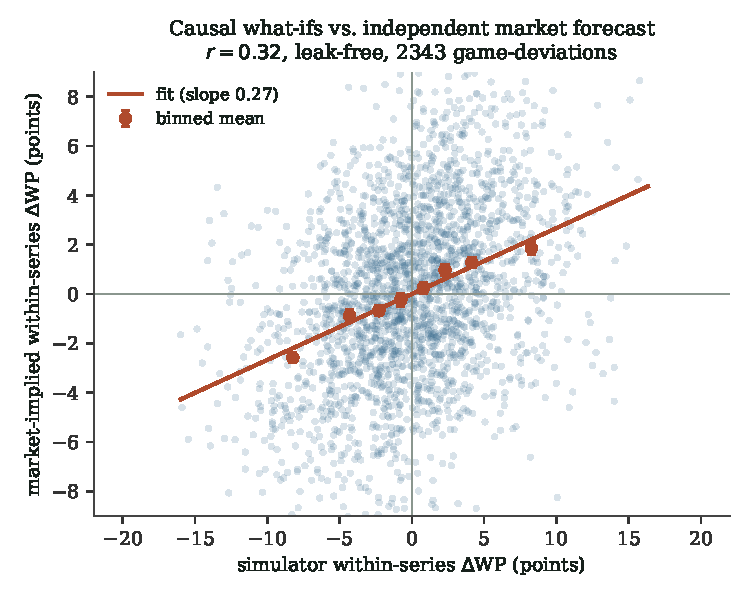
\includegraphics[width=\linewidth]{figs/fig1_validation.pdf}
\caption{Simulator within-series win-probability deltas versus an independent market's, on 2{,}343
game-deviations ($R{=}500$). Team strength and home field are differenced out, so the variation is the
starter and lineup matchup, what a counterfactual isolates. Direction is validated and leak-free
($r{=}0.32$); the fitted slope gives the magnitude calibration.}
\label{fig:val}
\end{figure}

\begin{figure}[t]
\centering
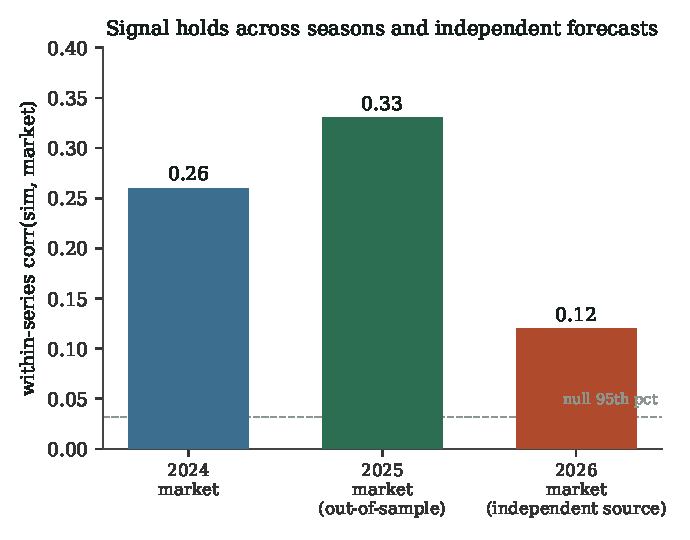
\includegraphics[width=0.92\linewidth]{figs/fig2_crossmarket.pdf}
\caption{The validation is not a single-season, single-source artifact: it holds a full season
out-of-sample and against a second, independent market forecast, degrading gracefully with model
staleness.}
\label{fig:cross}
\end{figure}

\begin{table}[t]
\centering\footnotesize
\setlength{\tabcolsep}{5pt}
\caption{Validation summary. Leak-free within-series agreement between the simulator's causal deltas and
an independent market, across seasons and sources; both input channels are priced.}
\label{tab:val}
\begin{tabular}{@{}llcc@{}}
\toprule
\textbf{Season} & \textbf{Rates} & \textbf{Source} & \textbf{corr} \\
\midrule
2024 & $\le$2023 & market A & 0.26 \\
2025 (out-of-sample) & $\le$2024 & market A & \textbf{0.33} \\
2026 & $\le$2023 (stale) & market B & 0.12 \\
\midrule
\multicolumn{3}{@{}l}{team fixed-effects residual (2024)} & 0.33 \\
\multicolumn{3}{@{}l}{pitching channel / hitting channel ($t$)} & 17.6 / 7.3 \\
\multicolumn{3}{@{}l}{magnitude calibration (slope)} & 0.33 \\
\bottomrule
\end{tabular}
\end{table}

\section{Grounding: what the simulator does and does not do}
\label{sec:bench}
A validated causal engine is only useful if its raw outputs are realistic. We benchmark them against the
baselines a reviewer would demand, and report where the simulator does \emph{not} lead
(Table~\ref{tab:bench}).

\textbf{Run-total distribution: a measured advantage.} The headline capability is a correlated
overdispersion a summed model cannot produce. Against an independent two-Poisson model with the identical
per-game means (so only the shape differs), the simulator matches reality's spread (variance $17.87$
versus $18.24$) and its central intervals cover at nominal rates, while the summed model badly
under-covers (Fig.~\ref{fig:cov}; randomized-PIT KS $0.049$ versus $0.144$~\cite{gneiting}). The
realistic bullpen earns this: without the hook model the same simulator covered only $0.74$ at the
$80\%$ level. A league negative-binomial matches the marginal but gives every matchup the identical
distribution, which is exactly what the simulator provides and it cannot. Figure~\ref{fig:rundist} shows
the effect directly: the simulator tracks the real game-total distribution including its heavy blowout
tail, while an independent-Poisson model with the same mean is too peaked in the middle and too thin in
the tail.

\begin{figure}[t]
\centering
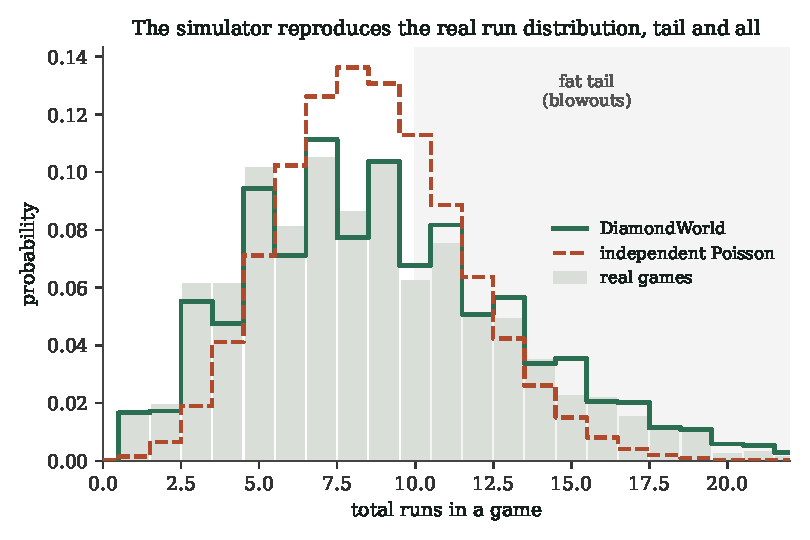
\includegraphics[width=\linewidth]{figs/fig7_rundist.pdf}
\caption{Game-total run distribution. The simulator (green) matches real games (bars) across the whole
range; an independent-Poisson model with the same mean (dashed) concentrates in the middle and misses
the fat blowout tail that drives leverage and bullpen decisions.}
\label{fig:rundist}
\end{figure}

\textbf{Win probability: calibrated, not sharp.} Point win probability is honestly \emph{not} the
simulator's edge. It is well calibrated (ECE $0.034$ over the full season) but discriminates less than a
simple team-strength baseline: AUC $0.572$ versus Log5~\cite{james} $0.617$ and the market $0.614$. A
per-plate-appearance process washes team-level talent toward a coin flip. The simulator's value is the
distribution and the counterfactuals, not the point estimate, and we verified one cannot fuse the two:
blending the simulator's win probability with Log5 recovers Log5.

\textbf{Player realism} (Fig.~\ref{fig:players}). The players inside the simulator are on par with a
standard projection baseline: cross-player rate correlation $0.611$, versus Marcel~\cite{tango} $0.626$
and Steamer's actual preseason projections $0.671$ (recovered from a public archive for a direct
comparison). It does not out-project a dedicated system, and it need not: the game-level analyses only
require realistic players, which these are.

\begin{table*}[t]
\centering\footnotesize
\setlength{\tabcolsep}{10pt}
\caption{Benchmarks against the baselines that matter. The simulator leads on the run-total distribution,
trails a one-line team-strength baseline on point win probability, and is competitive on player realism.
Bold marks the best in each row.}
\label{tab:bench}
\begin{tabular}{@{}lcccl@{}}
\toprule
\textbf{Task / metric} & \textbf{DiamondWorld} & \textbf{Independent / summed} & \textbf{Team-strength} & \textbf{Reference} \\
\midrule
Run-total variance & 17.87 & 8.99 (2-Poisson) & & 18.24 (real)\\
Run-total 80\% interval coverage & \textbf{0.82} & 0.66 (2-Poisson) & & 0.80 (nominal)\\
Run-total randomized-PIT KS & \textbf{0.049} & 0.144 (2-Poisson) & & 0 (ideal)\\
Win probability AUC & 0.572 & & \textbf{0.617} (Log5) & 0.614 (market)\\
Win probability ECE & \textbf{0.034} & & 0.019 (Log5) & 0.019 (market)\\
Player rate corr.\ (avg) & 0.611 & & 0.626 (Marcel) & \textbf{0.671} (Steamer)\\
\bottomrule
\end{tabular}
\end{table*}

\begin{figure}[t]
\centering
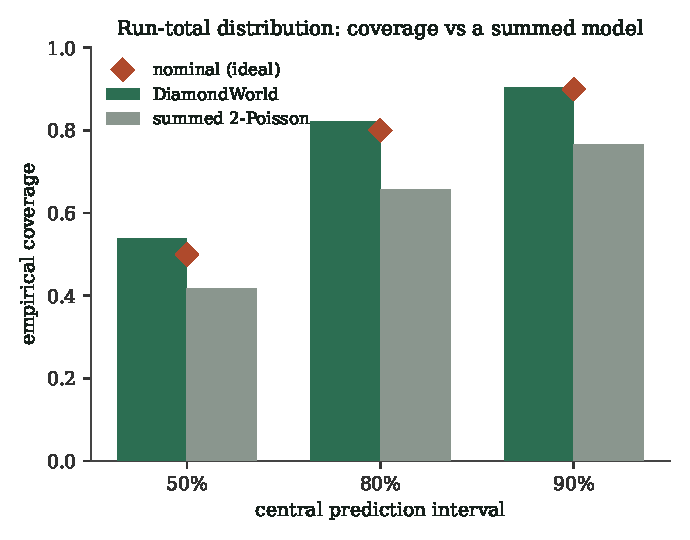
\includegraphics[width=0.92\linewidth]{figs/fig3_coverage.pdf}
\caption{Per-game run-total interval coverage over 2{,}376 games. The simulator is near-nominal; an
independent summed projection with the same means cannot produce the real spread.}
\label{fig:cov}
\end{figure}

\begin{figure}[t]
\centering
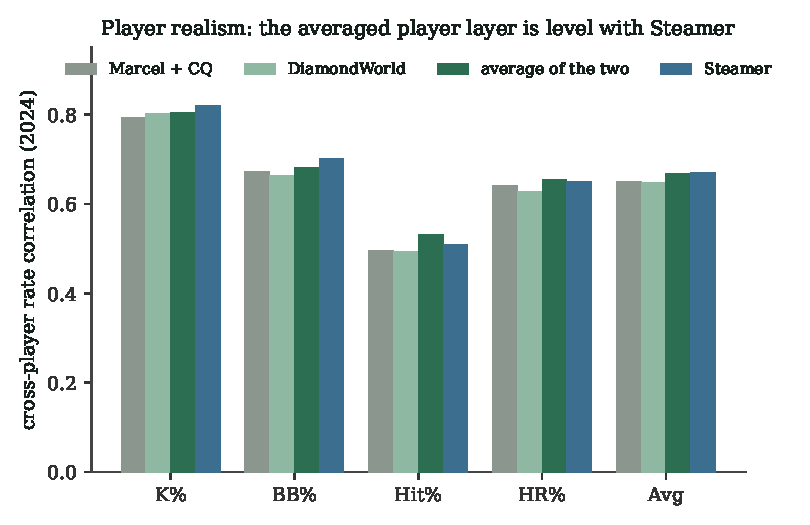
\includegraphics[width=\linewidth]{figs/fig4_players.pdf}
\caption{The simulator's players are as realistic as a standard projection baseline (Marcel) and within
a few points of a professional system (Steamer).}
\label{fig:players}
\end{figure}

\begin{figure}[t]
\centering
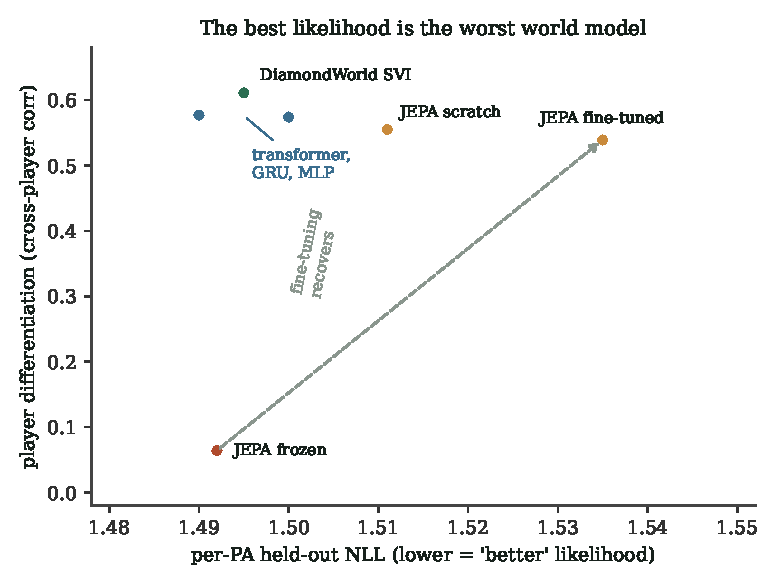
\includegraphics[width=0.95\linewidth]{figs/fig5_metric.pdf}
\caption{The best held-out likelihood is the worst world model. A frozen self-supervised probe minimizes
NLL and cannot tell players apart; fine-tuning the same encoder recovers differentiation, and the
generative model leads.}
\label{fig:metric}
\end{figure}

\section{A worked decision}
Consider a contending club weighing a deadline acquisition of a front-line starter. Run naively, the
simulator reports the swap is worth $9.8$ points of win probability in a representative game, which,
compounded over roughly thirty remaining starts, would read as a very large edge and could justify a
substantial overpay. The market-calibrated engine instead reports about $3.3$ points per start
(\S\ref{sec:val}), and it reports it with a credible band from the roster-uncertainty decomposition
rather than a single number. The calibration is the difference between a defensible valuation and a
threefold overstatement, and because the same machinery is validated to agree with the market on the
changes the market prices, the club can extend it with confidence to the changes the market does not
price directly: lineup and rest decisions, leverage planning, and bullpen deployment read against the
true, overdispersed run distribution rather than its mean.

\section{Limitations}
We are explicit about the boundaries. First, the raw counterfactual magnitudes overstate real effects by
about $3\times$ and must be market-calibrated (\S\ref{sec:val}). Second, point win probability is less
sharp than a one-line team-strength baseline (\S\ref{sec:bench}). Third, the out-of-sample validation
uses the model's rate features (its inputs) rather than a full re-simulation of each historical game,
and the later-season slice is coverage-limited by stale rates. Fourth, the simulator's mean runs about
$0.4$ high, a recalibration-scale artifact worth re-tuning. None of these undercut the central result:
the causal directions and calibrated magnitudes agree with an independent market, leak-free and
out-of-sample.

\section{Discussion}
The contribution is not ``we built a good model,'' but a generative object whose \emph{causal} answers
are validated against how an independent, information-aggregating market prices real games, in direction
and calibrated magnitude, on pitching and hitting, out-of-sample across seasons and across more than one
source, together with a distributional capability (calibrated per-game run distributions) a summed
projection cannot provide, and an honest account of where the object does not lead. To our knowledge this
is the first market-validated causal simulator for baseball. The practical implication is that a front
office can read the simulator's calibrated what-ifs, acquisition impact, lineup and rest decisions,
leverage and bullpen planning under the true run distribution, knowing that the same machinery agrees
with the market on the changes it prices and extends coherently to those it does not. All code and the
data-join pipelines are open-source.

{\footnotesize
\vspace{0.4ex}\noindent\textbf{Reproducibility.} Model, simulator, market joins, and every figure are
reproducible from the released code: \texttt{scenario\_sim.py}, \texttt{run\_pregame\_sim.py},
\texttt{simulator\_benchmarks.py}, \texttt{counterfactual\_validation.py}, \texttt{whatif\_channels.py},
\texttt{season\_market\_validation.py}, and \texttt{make\_figures.py}.
}

\begin{thebibliography}{99}\footnotesize
\bibitem{tango} T.~Tango. The Marcel the Monkey Forecasting System. tangotiger.net, 2004.
\bibitem{bukiet} B.~Bukiet, E.~R.~Harold, and J.~L.~Palacios. A Markov chain approach to baseball.
\emph{Operations Research}, 45(1):14--23, 1997.
\bibitem{nakahara} H.~Nakahara, K.~Takeda, and K.~Fujii. Estimating the effect of team hitting strategies
using counterfactual virtual simulation in baseball. \emph{arXiv:2206.01871}, 2022.
\bibitem{cervone} D.~Cervone, A.~D'Amour, L.~Bornn, and K.~Goldsberry. A multiresolution stochastic
process model for predicting basketball possession outcomes. \emph{Journal of the American Statistical
Association}, 111(514):585--599, 2016.
\bibitem{lecun} Y.~LeCun. A path towards autonomous machine intelligence. OpenReview, 2022.
\bibitem{assran} M.~Assran, Q.~Duval, I.~Misra, P.~Bojanowski, P.~Vincent, M.~Rabbat, Y.~LeCun, and
N.~Ballas. Self-supervised learning from images with a joint-embedding predictive architecture. In
\emph{CVPR}, pages 15619--15629, 2023.
\bibitem{bardes} A.~Bardes, J.~Ponce, and Y.~LeCun. VICReg: Variance-invariance-covariance regularization
for self-supervised learning. In \emph{ICLR}, 2022.
\bibitem{phan} D.~Phan, N.~Pradhan, and M.~Jankowiak. Composable effects for flexible and accelerated
probabilistic programming in NumPyro. \emph{arXiv:1912.11554}, 2019.
\bibitem{jax} J.~Bradbury, R.~Frostig, P.~Hawkins, et~al. JAX: Composable transformations of Python+NumPy
programs, 2018.
\bibitem{gneiting} T.~Gneiting and A.~E.~Raftery. Strictly proper scoring rules, prediction, and
estimation. \emph{Journal of the American Statistical Association}, 102(477):359--378, 2007.
\bibitem{james} B.~James. \emph{The Bill James Baseball Abstract}. Ballantine Books, 1984.
\end{thebibliography}

\end{document}
